\chapter{Произвольное пространство элементарных событий. Случайные величины и векторы}
\setcounter{equation}{0}
\section{Аксиомы теории вероятностей. Вероятностное пространство}
\begin{definition}
	Пусть $\Omega = \{\omega\}$. Набор подмножеств $\Omega$ $\mathcal{A}$ называется алгеброй, если
	\begin{enumerate}
		\item $\Omega \in \mathcal{A}$
		\item $\left.
			      \begin{aligned}
				      A \subset \Omega, B \subset \Omega \\
				      A \in \mathcal{A}, B \in \mathcal{A}
			      \end{aligned}
			      \right\} \Rightarrow A + B \in \mathcal{A}, A \cdot B \in \mathcal{A}$
		\item $\left.
			      \begin{aligned}
				      A \subset \Omega \\
				      A \in \mathcal{A}
			      \end{aligned}
			      \right\} \Rightarrow \overline{A} \in \mathcal{A}$
	\end{enumerate}
\end{definition}
\begin{definition}
	Набор подмножеств исходного множества $\Omega = \{\omega\}$ --- $\mathcal{F}$ называется $\sigma$-алгеброй, если он является алгеброй и:
	\[
		A_1, A_2, \dots, A_i, \dots A_k \subset \Omega \; \forall k,
	\]
	\[
		A_i \in \mathcal{F} \Rightarrow \sum\limits_{i=1}^\infty A_i \in \mathcal{F}, \; \prod\limits_{i=1}^\infty A_i \in \mathcal{F}.
	\]
\end{definition}
\subsection{Аксиомы Колмогорова}
$\big<\Omega, \mathcal{F}, \Prob \big>$ --- измеримое пространство.
\begin{enumerate}
	\item \textbf{Аксиома алгебры событий.} Заданы множества элементарных событий $\Omega = \{\omega\}$. На $\Omega$ выделена $\sigma$-алгебра $\mathcal{F}$, её элементы --- случайные события.
	\item \textbf{Аксиома существования алгебры событий.} Любому случайному событию $A \in \mathcal{F}$ сопоставлено неотрицательное число, называемое вероятностью этого события, $\forall A \in \mathcal{F}: \Prob(A) \geq 0$.
	\item \textbf{Аксиома нормированности.} $\Prob(\Omega) = 1$.
	\item \textbf{Аксиома аддитивности вероятности.} Если \\
	$A, B \in \mathcal{F}, A \times B = \emptyset$ $\Rightarrow$ $\Prob(A + B) = \Prob(A) + \Prob(B)$. \\
	      \begin{conclusion}
		      $A_1, \dots, A_n \in \mathcal{F}$: $A_i \times A_j \not = \emptyset$, $i \not= j$, $i, j = \To n$ $\Rightarrow$ $\Prob(\sum\limits_{i=1}^n A_i) = \sum\limits_{i=1}^n \Prob(A_i)$.
	      \end{conclusion}
	\item $A_1, \dots, A_n, \dots, \underset{i \not= j, i,j = 1, 2, \ldots}{A_i \in \mathcal{F} : A_iA_j} = \emptyset$ (попарно несовместны) $\Rightarrow$ $\Prob(\sum\limits_{i=1}^\infty A_i) = \sum\limits_{i=1}^\infty \Prob(A_i)$. \\ $\Prob$ -- нормированная счётно-аддитивная мера
\end{enumerate}
Рассмотрим монотонную случайную последовательность событий $A_1, \dots, A_n, \dots$
\begin{equation}\label{2-1-1}
	A_1 \subset A_2 \subset \dots \subset A_n \subset \dots, \overset{\forall n \in \mathbb{N}}{A_n \subset A_{n+1}}
\end{equation}
\begin{equation}\label{2-1-2}
	A_1 \supset A_2 \supset \dots \supset A_n \supset \dots, \overset{\forall n \in \mathbb{N}}{A_n \supset A_{n+1}}
\end{equation}
Тогда
\[ A = \sum\limits_{i=1}^\infty A_i = \lim\limits_{n \to \infty} A_n \text{--- предел (\ref{2-1-1})}.
\]
\[ A = \prod\limits_{i=1}^\infty A_i = \lim\limits_{n \to \infty} A_n \text{--- предел (\ref{2-1-2})}.
\]
\begin{definition}
	Функция событий $Q(A)$ называется непрерывной, если для любой монотонной последовательности случайных событий выполняется равенство
	\[
		\lim\limits_{n \to \infty} Q(A_n) = Q(\lim\limits_{n \to \infty} A_n)
	\]
\end{definition}
\begin{enumerate}
	\setcounter{enumi}{4}
	\item[$5'.$] \textbf{Аксиома непрерывности.} Пусть $A_n$ --- монотонно убывающая последовательность случайных событий. \\ $[A_n \downarrow \emptyset] \Leftrightarrow A_{n+1} \subset A_n, n = 1, 2, \dots$ ($\prod\limits_{i=1}^n A_i = \emptyset$ --- предел невозможен). Тогда
	      \[
		      \lim\limits_{n \to \infty} \Prob(A_n) = 0.
	      \]
\end{enumerate}

\begin{theorem}
	Вероятность является непрерывной функцией событий.
\end{theorem}
\begin{proof}
	\begin{description}[leftmargin = 0cm]
		\item Из аксиомы (5) $\Rightarrow$ (5') \\
		      Пусть $B_n \downarrow \emptyset$, $A_n = B_n \cdot \overline{B_{n+1}}$, где $n = 1,2, \dots$ \\
		      \[
			      B_1 = \sum\limits_{k=1}^\infty A_k, \; B_n = \sum\limits_{k=n}^\infty A_k,
		      \]
		      \[
			      \Prob(B_1) = \Prob(\sum\limits_{k=1}^\infty A_k) = \sum\limits_{k=1}^\infty \Prob(A_k)
		      \]
		      \[ \Prob(B_n) = \Prob(\sum\limits_{k=n}^\infty A_k) = \underbrace{\sum\limits_{k=n}^\infty \Prob(A_k)}_{n \to \infty} \to 0 \]
		      \[ \lim\limits_{n \to \infty} \Prob (B_n) = 0\]
		\item Из аксиомы (5') $\Rightarrow$ (5) \\
		      Пусть имеется множество попарно несовместных событий ${\{A_n\}}_{n = 1, 2, \dots}$.
		      \[ B_n = \sum\limits_{k=n+1}^\infty A_k, A = \sum\limits_{k=1}^\infty A_k \]
		      \[ A = A_1 + \ldots + A_n + B_n \]
		      \[ \Prob(A) = \sum\limits_{k=1}^n \Prob(A_k) + \underbrace{\Prob(B_n)}_{\to 0} \]
		      \[ B_{n+1} \subset B_n \]
		      \[ B_n \Rightarrow A_i, i > n \Rightarrow A_{i+1} \text{ не наступило} \Rightarrow \text{не наступило } B_i, \dots \]
		      \[ \prod\limits_{i=1}^\infty B_i = 0 \]
	\end{description}
\end{proof}
\section{Свойства вероятности}
\begin{enumerate}
	\item Вероятность невозможного события $\Prob(\emptyset) = 0$
	      \begin{proof}
		      $ \emptyset+ \Omega = \Omega $
		      \[
			      1 = \Prob(\Omega) = \Prob(\emptyset + \Omega) \overset{(\text{акс. } 4)}{=} \Prob(\emptyset) + \underbrace{\Prob(\Omega)}_{= 1} = 1
		      \]
	      \end{proof}
	\item $\Prob(\overline{A}) = 1 - \Prob(A)$
	      \begin{proof}
		      \[
			      1 = \Prob(\Omega) = \Prob(A + \overline{A}) \overset{(\text{акс. } 4)}{=} \Prob(A) + \Prob(\overline{A}) = 1
		      \]
	      \end{proof}
	\item $A \subset B$ $\Rightarrow$ $\Prob(A) \leqslant \Prob(B)$
	      \begin{proof} $B = A \times B + \overline{A} \times B \overset{A \subset B}{=} A + \overline{A} \times B$
		      \[
			      \Prob(B) = \Prob(A + \overline{A} \times B) \overset{(\text{акс. } 4)}{=} \Prob(A) + \Prob(\overline{A} \times B)
		      \]
	      \end{proof}
	\item $\Prob(A + B) = \Prob(A) + \Prob(B) - \Prob(A \times B)$
	      \begin{proof}
		      \[
			      A + B = A + \overline{A} \times B, B = A \times B + \overline{A} \times B \Rightarrow
		      \]
		      \[
			      \Prob(A + B) \overset{(\text{акс. } 4)}{=} \Prob(A) + \Prob(\overline{A} \times B)
		      \]
		      \[
			      \Prob(B) = \Prob(A \times B) + \Prob(\overline{A} \times B)
		      \]
	      \end{proof}
	\item $\Prob(A+B) \leqslant \Prob(A) + \Prob(B)$ \\
	      Также можно показать, что:
		  \[
	      		\Prob(\sum\limits_{k=1}^n A_k) \leqslant \sum\limits_{k=1}^n \Prob(A_k)
	      \]
	      \[
		      \Prob(\sum\limits_{k=1}^\infty A_k) \leqslant \sum\limits_{k=1}^\infty \Prob(A_k)
	      \]
	\item $A_1, \dots, A_n$:
		  \[ \Prob(\sum\limits_{k=1}^\infty A_k) = \sum\limits_{k=1}^\infty \Prob(A_k) - \sum\limits_{k=1}^{n-1} \sum\limits_{i=k+1}^n \Prob(A_k \times A_j) + \ldots \]
	      \[ \ldots + (-1)^{n-1} \cdot \Prob(\prod\limits_{k=1}^n A_k) \]
	      Пусть $B = \sum\limits_{k=1}^{n+1} A_k$. Тогда
	      \[
		      \Prob(\sum\limits_{k=1}^{n+1} A_k) = \Prob(A_{n+1} + \sum\limits_{k=1}^n A_k)
	      \]
	\item \textbf{Теорема.} Пусть имеется $k$ попарно несовместных и составляющих полную группу благоприятных к событию $A$ исходов из всех исходов $n$, $\{ E_1, \dots, E_n\}_{\underset{i, j = 0, 1, \ldots}{E_i \times E_j = \emptyset, i \not = j}}$, $\sum\limits_{i=1}^n E_i = \Omega$. Тогда
	      \[
		      \Prob(A) = \frac{k}{n}
	      \]
	      \begin{proof}
		      $A = \sum\limits_{s=1}^k E_{i_s}$
		      \[
			      1 = \Prob(\sum\limits_{i=1}^n E_i) \overset{(\text{акс. } 4)}{=} \sum\limits_{i=1}^n \Prob(E_i) = n \cdot \Prob(E_i), \Prob(E_i) = \frac{1}{n}
		      \]
		      \[
			      \Prob(A) = \Prob(\sum\limits_{s=1}^k E_{i_s}) \overset{(\text{акс. } 4)}{=} \sum\limits_{s=1}^k \Prob(E_{i_s}) = \frac{k}{n}
		      \]
		      \[
			      \Omega = \{E_1, \dots, E_n\}, \mathcal{F} = \{A = E_{i_1} + \ldots + E_{i_k}\}, k \leqslant n
		      \]
		      \[
			      \Prob(A) = \frac{k}{n}
		      \]
	      \end{proof}
	      \setcounter{enumi}{7}
	\item $0 \leqslant \Prob(A) \leqslant 1, A \in \mathcal{F}$
	      \[
		      0 \leqslant \Prob(\overline{A}) = 1 - \Prob(A) \Rightarrow \Prob(A) \leqslant 1
	      \]
	      Для условных вероятностей:
	      \[
		      \Prob(A|B) \overset{\textrm{def}}{=} \frac{\Prob(A \times B)}{\Prob(B)}
	      \]
	      $\Prob(B) > 0$
	      \[
		      \Prob(\Omega | B) = \frac{\Prob(\Omega \times B)}{\Prob(B)} = \frac{\Prob(B)}{\Prob(B)} = 1.
	      \]
	      Аксиома нормированности выполнена. \\
	      Пусть $A_1, \ldots, A_n, \ldots$ --- не более чем счётный набор, $A_i \times A_j = \emptyset, i \not = j; i,j = \To n$ \\
	      Пусть также имеется событие $B$, $\Prob(B) > 0$.
	      \[
		      \Prob \left( \sum\limits_{n} A_n | B \right) = \frac{\Prob((\sum\limits_{n} A_n) \times B)}{\Prob(B)} = \frac{\sum\limits_{n} \Prob(A_n \times B_n)}{\Prob(B)} =
	      \]
	      \[
		      \overset{(\text{акс. } 4, 5)}{=} \sum\limits_{n} \Prob(A_n | B)
	      \]

	\item $\mathcal{F}_* = \{\emptyset, \Omega\}$ --- наименьшая $\sigma$-алгебра, $\mathcal{F}^* = \{A: A \subseteq \Omega \}$ --- наибольшая $\sigma$-алгебра. \\
	      Пусть имеется $n$ испытаний в эксперименте с подбрасыванием монет. Построим измеримое пространство

	      \[
		      \Omega = \{ \text{О, Р} \}, \mathcal{F}^{*} : \{ \text{О} \}, \{ \text{Р} \}, \{ \text{О + Р} \}, \emptyset
	      \]

	      Зададим вероятности событий (О --- орёл, Р --- решка)
	      \[
		      \Prob(\text{О}) = p, \Prob(\text{Р}) = q: p + q = 1.
	      \]
	      Создано вероятностное пространство. \\
	      В случае несчётного пространства элементарных событий набор всех подмножеств элементарных событий и построенная $\sigma$-алгебра не будет удовлетворять испытанию, чтобы задать вероятность на этом множестве. \\
	      Можем основываться на определённом наборе подмножеств $\Omega$.
	      \begin{definition}
		      Наименьшая $\sigma$-алгебра, содержащая заданный класс подмножеств $\Omega$, называется $\sigma$-алгеброй, порождаемой этим классом.
	      \end{definition}

	      \begin{example}
		      $\Omega = [0, 1]$. Пусть $\sigma$-алгебра $\mathcal{F}$ составляет все подмножества, для которых можно определить длину, $\{\omega\}$ --- точки отрезка $[0, 1]$.
		      \[
			      A \in \mathcal{F} : \Prob(A) = \mu (A) \text{ --- длина некоторого отрезка, мера}
		      \]
		      При не более чем счётном пространстве событий мы говорим о дискретных пространствах. В противном случае --- о непрерывно измеримых.
	      \end{example}
\end{enumerate}
\section{Способы задания вероятностных мер на измеримом пространстве $(\mathbb{R}^1, \mathcal{B} (\mathbb{R}^1) )$}
$\mathbb{R}^1 = (-\infty; +\infty)$ --- вещественная прямая. Рассмотрим на $\mathbb{R}^1$ интервал такого вида:
\[
	\{ (a, b] = \{x \in \mathbb{R}^1 | a < x \leqslant b \} \}
\]
\[
	- \infty \leqslant a < b < +\infty
\]
Рассмотрим множество таких интервалов.
\begin{definition}
	Наименьшая $\sigma$-алгебра, содержащая систему вида (*), называется борелевской алгеброй множеств вещественной прямой.
\end{definition}
\begin{definition}
	Борелевские множества -- элементы $\mathcal{B}(\mathbb{R}^1)$. Они же и являются событиями.
\end{definition}
Заметим, что интервалы
\[
	(a, b) = \sum\limits_n (a, b - \frac{1}{n}]
\]
Отрезки:
\[
	[a, b] = \prod\limits_n (a - \frac{1}{n}, b]
\]
Например, точка $a$:
\[
	\{ a \} = \prod\limits_n (a - \frac{1}{n}, a]
\]
Остановимся на рассмотрении $(a, b]$, хотя и другие виды ведут к той же борелевской алгебре. \\

Построим вероятностное пространство на основе этого измеримого пространства. Пусть $\Prob$ -- вероятность, заданная на борелевском множестве. Возьмём борелевское множество:
\[
	B = (- \infty, x], x \in \mathbb{R}^1
\]
Положим
\begin{equation}\label{2-3-1}
	F (x) = \Prob \{ (- \infty, x] \}
\end{equation}
Так определённая функция, оказывается, обладает следующими свойствами:
\begin{enumerate}
	\item $F(x)$ монотонно не убывает на $\mathbb{R}^1$.
	      \begin{proof}
		      Пусть $x_1 < x_2$. Тогда соответствующее событие
		      \[
			      (-\infty, x_1] \subset (-\infty, x_2] \Rightarrow \Prob \{ (-\infty, x_1] \} \leqslant \Prob \{ (-\infty, x_2] \}
		      \]
		      Итак, функция монотонно неубывающая
		      \[
			      F(x_1) \leqslant F(x_2), \forall x_1, x_2 \in \mathbb{R}^1, x_1 < x_2
		      \]
	      \end{proof}
	\item Пусть $\lim\limits_{x \to -\infty} F(x) = F(-\infty)$, $\lim\limits_{x \to +\infty} F(x) = F(+\infty)$, тогда $F(-\infty) = 0, F(\infty) = 1$.
	      \begin{proof}
		      В силу монотонности предел функции существует. Докажем, что $\underset{n = 1, 2, \ldots}{F(-n)} \underset{n \to \infty}{\rightarrow} 0.$ \\
		      Рассмотрим последовательность событий:
		      \[
			      \{ B_n = (-\infty, -n] \}
		      \]
		      \[
			      \left.
			      \begin{cases}
				      B_{n+1} \subset B_n \\
				      \lim\limits_{n \to \infty} B_n = \prod\limits_n B_n = \emptyset
			      \end{cases}
			      \right\}
			      B_n \downarrow \emptyset
		      \]
		      Для этой последовательности (по акс. непрерывности)
		      \[
			      \lim\limits_{n \to \infty} \underbrace{\Prob(B_n)}_{F(-n)} = 0
		      \]
		      %TODO: для второго предела
	      \end{proof}
	\item $F(x)$ непрерывна справа и имеет предел слева $\forall x \in \mathbb{R}^1$
	      \[
		      \lim\limits_{y \uparrow x} F(y) = F(x - 0), \lim\limits_{y \downarrow x} F(y) = F(x + 0)
	      \]
	      Тогда $\forall x \in \mathbb{R}^1: F(x+0) = F(x)$, $F(x) - F(x-0) \geqslant 0$.
	      \begin{proof}
		      Рассмотрим монотонную последовательность $x_n \downarrow x$. Введём последовательность событий
		      \[
			      \{ \underset{n = 1, 2, \ldots}{B_n} = (-\infty, x_n] \}, B = (-\infty, x]
		      \]
		      Рассмотрим предел $\{ B_n \}_{n = 1, 2, \ldots}$
		      \[
			      \prod\limits_n B_n = B
		      \]
		      Перейдём к вероятностям:
		      \[
			      \lim\limits_{n \to \infty} \Prob(B_n) = \Prob(\lim\limits_{n \to \infty} B_n) = \Prob(B)
		      \]
		      \[
			      \Prob(B) = F(x) \Rightarrow \lim\limits_{n \to \infty} F(x_n) = F(x)
		      \]
	      \end{proof}
\end{enumerate}
\begin{definition}
	Любая функция, удовлетворяющая условиям (1, 2, 3), называется функцией распределения на вещественной прямой.
\end{definition}
Оказывается, что распределение вероятности имеет не более чем счётное количество скачков (разрывов функции).
Функция распределения может иметь не более
\begin{itemize}
	\item 1 скачка размером $\frac{1}{2}$,
	\item 2 скачков размером $\frac{1}{4}$,
	\item n скачков размером $\frac{1}{2^n}$.
\end{itemize}
Функция распределения непрерывна $\Leftrightarrow$ вероятность точечного события равна нулю.
\[
	\forall x \in \mathbb{R}^1: F(x) \text{ непрерывна } \Leftrightarrow \Prob(\{ x \}) = 0
\]
\begin{proof}
	\[
		F(x) - F(x-0) = \lim\limits_{n \to \infty} (F(x) - F(x - \frac{1}{n})) =
	\]
	\[ = \lim\limits_{n \to \infty} [\{ \Prob(-\infty, x] - \Prob(-\infty, x - \frac{1}{n}] \}] \]
	Представим как сумму двух несовместных событий
	\[
		(-\infty, x - \frac{1}{n}] + (x - \frac{1}{n}, x]
	\]
	\[
		\Prob \{ (-\infty, x] \} = \Prob \{ (-\infty, x - \frac{1}{n} ] \} + \Prob \{ (x - \frac{1}{n}, x ]
	\]
	\[
		\lim\limits_{n \to \infty} \Prob \{ (x - \frac{1}{n}, x] \} = \Prob \{ \prod\limits_n (x - \frac{1}{n}, x] \} = \Prob \{ x \}.
	\]
	Итак, $F(x) - F(x-0) = \Prob \{ x \}$.
\end{proof}
\[
	\{ (a, b] \}, -\infty \leqslant a < b < +\infty
\]
В зависимости от выбора вида интервала свойства (1, 2, 3) изменяются подобно изменению интервала.
\begin{theorem}
	Пусть $F(x)$ --- некоторая функция распределения. Тогда на измеримом пространстве $(\mathbb{R}^1, \mathcal{B}(\mathbb{R}^1))$ $\exists \ !$ вероятностная мера $P$, такая, что
	\[
		P: -\infty \leqslant a < b < +\infty
	\]
	\begin{equation}\label{2-3-2}
		P \{ (a, b] \} = F(b) - F(a)
	\end{equation}
	Соотношения (\ref{2-3-1}) и (\ref{2-3-2}) устанавливают взаимно однозначное соответствие между функцией распределения и вероятностной мерой.
\end{theorem}
\begin{theorem}
	(Каратеодори). Пусть имеется вероятностное пространство в широком смысле $(\Omega, \mathcal{A}, P)$. Тогда существует единственная вероятностная мера $Q$ на $\sigma$-алгебре $\mathcal{F} = \sigma(\mathcal{A})$ --- порождённая $\mathcal{A}$, что:
	\[
		Q(A) = P(A), A \in \mathcal{A}.
	\]
\end{theorem}
\begin{conclusion}
	Любое вероятностное пространство в широком смысле автоматически определяет вероятностное пространство.
\end{conclusion}
Из этого следует, что для определения вероятности достаточно задать вероятности интервалов. \\
Рассмотрим алгебру, элементами которой является сумма непересекающихся интервалов.
\[
	\mathcal{A} : A = \sum\limits_{k = 1}^n (a_k, b_k], a_k < b_k
\]
На этих множествах определим функцию множеств
\[
	\Prob_0 (A) = \sum\limits_{k = 1}^n [ F(b_k) - F(a_k) ] \text{ (вероятности интервалов)}
\]
Проверим выполнение аксиом
\begin{itemize}
	\item Акс. 2, 3, 4 выполняются, что почти очевидно.
	\item Акс. 5 также выполняется, см [1]. %TODO: bibtex
\end{itemize}
\[
	\sigma(\mathcal{A}) = \mathcal{B}(\mathbb{R}^1)
\]
Итак, для любой функции распределения существует единственная вероятностная мера. Таким образом строим вероятностное пространство $(\mathbb{R}^1, \mathcal{B} (\mathbb{R}^1), P)$.

\subsection{Меры на измеримых пространствах}
\subsubsection{Дискретные вероятностные меры}
Пусть $F(x)$ --- функция распределения $x_1 < x_2 < \ldots < \ldots$
\[
	\Delta F(x) = F(x) - F(x-0),
\]
\[
	\Prob(x_k) = \Delta F(x_k), k = 1, 2, \ldots
\]
\[
	\sum\limits_k \Prob(x_k) = 1
\]
Представим иллюстрацию ситуации
\begin{figure}[H]
	\begin{center}
	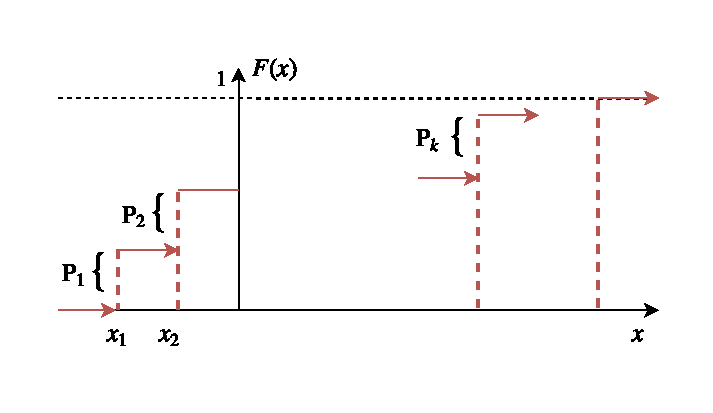
\includegraphics[width=\textwidth,height=\textheight,keepaspectratio]{Images/plot2-1.pdf}
	\end{center}
	\caption{Дискретный закон распределения вероятностей.}
\end{figure}

Такой набор чисел называется дискретным законом распределения вероятностей на вещественной прямой.
\begin{example}
	$\{ \Prob_k = \frac{1}{N} \}$ --- дискретный равномерный закон, $k = 1, \ldots, N$
\end{example}
\begin{example}
	$\{ p_1, p_2 \} : p_1 = 1 - p_2$ --- бернуллиевское дискретное распределение (часто обозначают как $p, q$).
\end{example}
\begin{example}
	${ \{ {\Prob}_{m}^{ (n) } \} }_{m = 0, 1, \ldots, n}$, $n$ --- число испытаний, $p$ --- вероятность появления успеха в каждом испытании. \\
	$\Prob_m^{(n)} = C_n^m \cdot p^m \cdot (1 - p)^{n-m}$ --- биномиальное дискретное распределение.
\end{example}
\begin{example}
	$\Prob_m = \frac{a^m}{m!} \cdot e^{-a}, a \in \mathbb{R}, a > 0, m = 0, 1, \ldots$ --- дискретный закон распределения Пуассона.
\end{example}
\subsubsection{Абсолютно непрерывные вероятностные меры}
Пусть $F(x)$ непрерывна $\forall x \in \mathbb{R}$, при этом существует вещественная неотрицательная кусочно-непрерывная функция плотности распределения вероятностей $f(x)$:
\[
	f(x) \geqslant 0 : F(x) = \int\limits_{-\infty}^x f(t) dt
\]
В этом случае
\[
	\Prob \{ (a, b] \} = \int\limits_a^b f(x) dx
\]
Очевидно, что если $x$ --- точка непрерывности $f(x)$, $x \in \mathbb{R}$, то
\[
	F'(x) = f(x)
\]

Плотностью распределения может быть любая кусочно-непрерывная, вещественнозначная функция $f(x)$, удовлетворяющая условию нормировки
\[
	\int\limits_{-\infty}^{+\infty} f(x) dx = 1
\]
\begin{example}
	Равномерное распределение на отрезке $[a, b]$, $a < b$
	\[
		f(x) = \frac{1}{b-a}, \; a \leqslant x \leqslant b
	\]
	Если $x < a$ или $x > b$, тогда
	\[
		f(x) = 0.
	\]
	Итак,
	\[
		f(x) =
		\begin{dcases*}
			\frac{1}{b-a}, \; a \leqslant x \leqslant b \\
			\;\;\;\;0, \; x < a \text{ или } x > b
		\end{dcases*}
	\]
\end{example}
\begin{example} Распределение Гаусса (нормальное)
	\[
		f(x) \sim N(a, \sigma), a \in \mathbb{R}, \sigma > 0
	\]
	Тогда
	\[
		f(x) = \underbrace{\frac{1}{\sqrt{2 \pi } \sigma}}_{\underset{\text{множитель}}{\text{норм.}}}\cdot e ^{-\frac{(x-a)^2}{2 \sigma^2}}
	\]
\end{example}
\begin{example} $\Gamma$-распределение \\
	Здесь в нормирующем множителе для плотности участвует $\Gamma$-функция
	\[
		f(x) =
		\begin{dcases*}
			\;\; 0, \; x \leqslant 0 \\
			\frac{\alpha^\lambda}{\Gamma(\lambda)} \cdot x^{\lambda - 1} \cdot e^{-\alpha x}, \; x > 0
		\end{dcases*}
	\]
	$\alpha$ --- параметр масштаба, $\lambda$ --- параметр формы. \\
	Экспоненциальное (показательное) распределение получаем при $\lambda = 1$:
	\[
		f(x) =
		\begin{cases}
			\alpha e^{-\alpha x}, \; x \geqslant 0 \\
			\;\;\; 0, \; x < 0
		\end{cases}
	\]
\end{example}
\subsubsection{Сингулярные вероятностные меры на $\mathbb{R}^1$}
Оказывается, $F(x)$ может быть непрерывной, но не иметь плотности. \\
$F(x)$ --- непрерывная функция распределения, функции плотности вероятности $f(x)$ не существует.
\begin{example} Канторова функция.
	\[
		F(x) =
		\begin{cases}
			0, x \leqslant 0 \\
			1, x \geqslant 1
		\end{cases}
	\]
	Представим, как ведёт себя функция распределения при $x \in (0, 1)$




	

	\begin{figure}[H]
	\begin{center}
	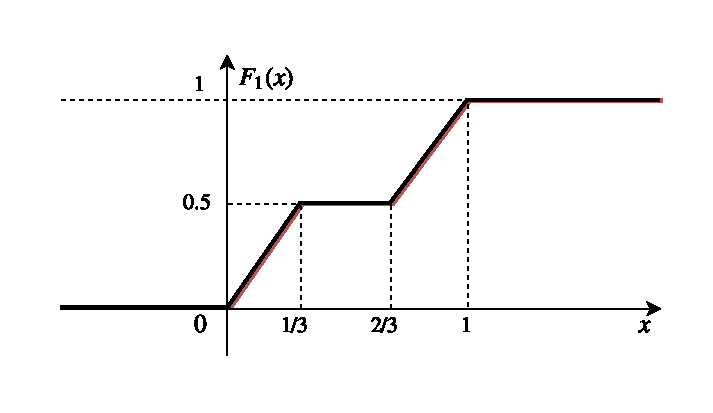
\includegraphics[width=\textwidth,height=\textheight,keepaspectratio]{Images/plot2-2.pdf}
	\end{center}
	\caption{$F_1(x)$ --- первое приближение Канторовой функции.}
	\end{figure}
	\begin{figure}[H]
	\begin{center}
	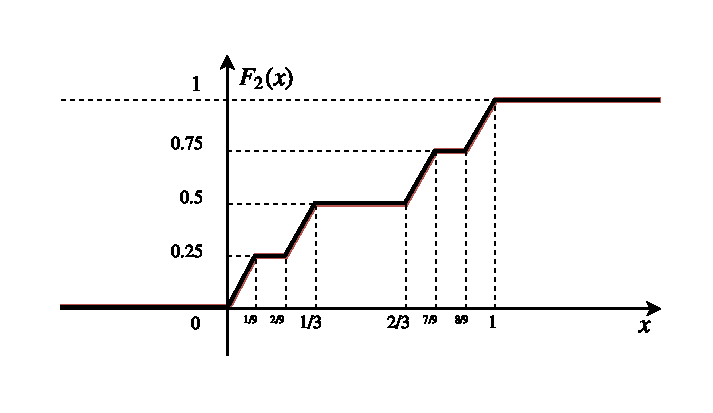
\includegraphics[width=\textwidth,height=\textheight,keepaspectratio]{Images/plot2-3.pdf}
	\end{center}
	\caption{$F_2(x)$ --- второе приближение Канторовой функции.}
	\end{figure}

	$F_n(x) \underset{n \to \infty}{\rightarrow} F(x)$ --- Канторова функция. \\
	Длина интервалов, на которой Канторова функция должна быть постоянна:
	\[
		\frac{1}{3} + \frac{2}{9} + \frac{4}{27} + \ldots = \frac{1}{3} \cdot \sum\limits_{n = 0}^\infty \left(\frac{2}{3}\right)^n = 1.
	\]
	$f(x)$ почти всюду обращается в 0, за исключением, может быть, множеств меры нуль. \\
	Функция называется сингулярной, поскольку она сингулярна по отношению к мере Лебега.
\end{example}
\begin{theorem} \textit{(Лебега)}.  
	Любая функция распределения в таком измеримом пространстве может быть представлена в виде:
	\[
		F(x) = p_1 F_1(x) + p_2 F_2(x) + p_3 F_3(x)
	\]
	где $p_i \geqslant 0, \sum\limits_{i=1}^3 p_i = 1$,
	\begin{itemize}
		\item $F_1 (x)$ --- дискретная функция распределения
		\item $F_2 (x)$ --- абсолютно непрерывная функция распределения
		\item $F_3 (x)$ --- сингулярная функция распределения
	\end{itemize}
\end{theorem}

\setcounter{equation}{0}
\section{Случайные величины}
\begin{definition}
	Вещественнозначная функция $\xi (\omega)$, определённая на измеримом пространстве $(\Omega, \mathcal{F})$, называется \textit{случайной величиной}, если
	\[
		\xi: \xi(\omega), \xi : \Omega \rightarrow \mathbb{R}^1
	\]
	\[
		\forall B \in \mathcal{B}(\mathbb{R}^1) \text{ --- борелевское множество из $\sigma$-алгебр $\mathcal{B}(\mathbb{R}^1)$}
	\]
	$\{ \omega : \xi(\omega) \in B \} \in \mathcal{F}$ --- такое множество всех элементов событий, для которых $\xi(\omega) \in B$ является событием.
	\begin{equation}
		\forall B : \xi^{-1}(B) = \{ \omega : \xi(\omega) \in B \} \in \mathcal{F}
	\end{equation}
\end{definition}
\begin{definition}
Вероятностная мера $\mathcal{P}_\xi$ на измеримом пространстве $(\mathbb{R}^1, \mathcal{B}(\mathbb{R}^1))$ такая, что:
\[
	\mathcal{P}_\xi (B) \overset{\textrm{def}}{=} \Prob \{ \omega : \xi (\omega) \in B \}
\]
называется \textit{распределением вероятностей случайной величины} $\xi$ на измеримом пространстве $(\mathbb{R}^1, \mathcal{B}(\mathbb{R}^1))$. \\
Эту вероятность далее будем обозначать как
\[
	\Prob \{ \xi \in B \}.
\]
\end{definition}
\begin{definition}
	$\forall x \in \mathbb{R}$ определим
	\[
		F_\xi (x) = \Prob \{ \omega : \xi (\omega) \leqslant x \} = \mathcal{P}_\xi \{ (-\infty, x] \}
	\]
	Здесь в качестве $B$ выступает интервал $(-\infty, x]$. \\
	$F_\xi (x)$ --- функция распределения случайной величины $\xi$. Обозначать далее будем как
	\[
		F_\xi (x) = \Prob \{ \xi \leqslant x \}
	\]
\end{definition}
Итак, каждая случайная величина порождает своё вероятностное пространство
\[
	\xi : \Omega \rightarrow \mathbb{R}^1 \rightarrow (\mathbb{R}^1, \mathcal{B}(\mathbb{R}^1), \mathcal{P}_\xi)
\]
Оказывается, множество пробных борелевских множеств можно существенно сузить, так как для определения вероятности достаточно задать вероятности интервалов. \\
Следовательно, функция распределения случайной величины полностью определяет распределение случайной величины. По $F_\xi (x)$ можно восстановить меру борелевского множества.\\
Рассмотрим типы случайных величин.
\begin{enumerate}
	\item Если возможные значения случайной величины образуют не более чем счётное множество, то такая случайная величина называется \textit{дискретной} случайной величиной. \\
	$\xi$ -- дискретна, $\{x_j \text{ --- возможное значение} \}_{j = 1, 2, \ldots}$, $\Prob \{ \xi = x_i \} = p_i$ --- вероятности. \\
	Можно вычислить все вероятности, связанные с $\xi$. $B$ -- борелевское множество, $B \in \mathcal{B} (\mathbb{R}^1)$, тогда
	\[
		\mathcal{P}_\xi (B) = \Prob \{ \xi \in B\} = \Prob \left(\sum\limits_{j : x_j \in B} (\xi = x_j)\right) = \sum\limits_{j : x_j \in B} \underset{p_j}{\Prob (\xi = x_j)}
	\]
	В этом случае
	\[
		F_\xi (x) = \sum\limits_{j : x_j \leqslant x} p_j \text{ --- ст. функция с разрывами в $x_j$}
	\]
	\item Случайная величина называется \textit{непрерывной}, если
	\[
		\exists f_\xi (x) \geqslant 0 : F_\xi (x) = \int\limits_{-\infty}^x f_\xi (t) dt
	\]
	\item Случайная величина называется \textit{сингулярной}, если функция её распределения $F_\xi (x)$ непрерывна, но функция плотности вероятности $f_\xi (x)$ не существует.
\end{enumerate}
Заметим, что в то время как любая случайная величина однозначно определяет свою функцию распределения, существует сколько угодно различных случайных величин, имеющих одну и ту же функцию распределения.
\begin{example} $x_i: -1, +1$; $p_i: \frac{1}{2}, \frac{1}{2}$; $\xi_i - \xi = \eta$

\begin{figure}[H]
	\begin{center}
	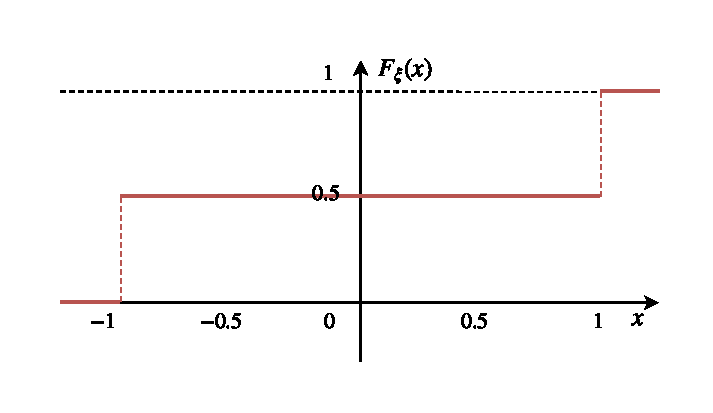
\includegraphics[width=\textwidth,height=\textheight,keepaspectratio]{Images/plot2-4.pdf}
	\end{center}
	\caption{Пример функции распределения.}
\end{figure}

	\[
		F_\eta = F_\xi =
		\begin{dcases*}
			0, \; x < -1 \\
			\frac{1}{2}, \; -1 \leqslant x < 1 \\
			1, \; x \geqslant 1
		\end{dcases*}
	\]
\end{example}
\begin{definition}
	Вещественнозначная функция $g(x)$, $x \in \mathbb{R}$ называется \textit{борелевской}, если для любого борелевского множества при отображении $g$ его полный прообраз также является борелевским множеством
	\[
		g : \mathbb{R}^1 \rightarrow \mathbb{R}^1, B \in \mathcal{B} (\mathbb{R}^1), g^{-1} (B) = \{ x, x \in \mathbb{R}^1 : g(x) \in B \}
	\]
\end{definition}
\begin{theorem}
	Пусть $\xi (\omega)$ --- случайная величина.
	\[
		\xi (\omega) : \Omega \rightarrow \mathbb{R}^1
	\]
	\[
		g(x) : \mathbb{R}^1 \rightarrow \mathbb{R}^1 \text{ --- борелевская функция}
	\]
	$\Omega = \{ \omega \}$ --- значение элементарного события. Тогда $\eta (\omega) = g (\xi (\omega))$ является случайной величиной.
\end{theorem}
\begin{proof}
	$B \in \mathcal{B} (\mathbb{R}^1)$
	\[
			\{ \omega : \eta (\omega) \in B \} = \{ \omega : g(\xi(\omega)) \in B \} = \{ \omega : \xi(\omega) \in g^{-1} (B) \} \in \mathcal {F}
	\]
	\[
		\xi \sim (\Omega, \mathcal{F})
	\]
	Это означает, что $\eta(\omega)$ --- случайная величина.
\end{proof}
Также возможно конструировать случайные величины как функции других случайных величин.
\subsection{Примеры случайных величин}
\begin{itemize}
	\item Пусть $A$ --- событие, $\xi(\omega) \equiv I_A (\omega) = \begin{cases}
		1, \omega \in A \\
		0, \omega \not \in A
	\end{cases} $ \\
	Задана функция-индикатор.
	\item Пусть испытание --- бросание игральной кости. Случайная величина --- число выпавших на верхней грани очков, всего возможно 6 значений, вероятность каждого -- $\frac{1}{6}$. Можем задать дискретное распределение с параметром 6.
	\item Распределение последовательности испытаний Бернулли. Пусть $\xi_i (\omega)$ --- число появления «успеха» в $i$-ом испытании.
%TODO: fix formatting
	\[
		\xi_i (\omega) : I_{A_i} (\omega) = \begin{cases}
		1, \omega \in A_i \\
		0, \omega \not \in A_i
	\end{cases} \text{--- Бернуллиевская случайная величина}
	\]
	Пусть $A_i$ --- в $i$-ом испытании «успех».
	\item Рассмотрим серию из $n$ испытаний Бернулли. $\mu_n$ --- число появления «успеха» в серии из $n$ испытаний. Пусть $p$ --- вероятность появления успеха в каждом из испытаний.
	\[
		{\{ \Prob \{ \mu_n = m \} = C_n^m p^m (1-p)^{n-m} \}}_{m = 0, \ldots, n}
	\]
	\item Пусть испытание --- «бросание» точки в отрезок случайным образом. $\Omega = \{ \omega \}$.
	\[
		\begin{cases}
			\Omega = [a, b] \text{ $a < b$ } \\
			\mathcal{F}
		\end{cases}
	\]
	\[
		\xi (\omega) = \omega
	\]
	\[
		F_\xi (x) \overset{\textrm{def}}{=} \Prob \{ \xi \leqslant x \} = \frac{x - a}{b - a}, \; a \leqslant x \leqslant b, \; \xi \in [a, x]
	\]
	\[
		F' (x) = \frac{1}{b-a}, x \in [a, b]
	\]
	\[
		x < a : \mathcal{F}_\xi (x) = 0, \; x > b : \mathcal{F}_\xi (x) = 1
	\]
\begin{figure}[H]
	\begin{center}
	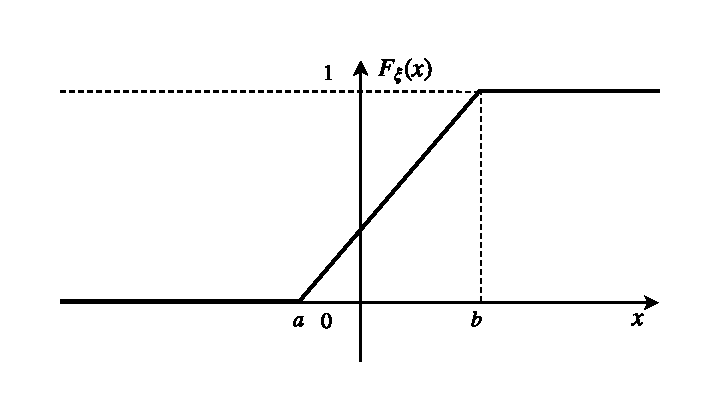
\includegraphics[width=\textwidth,height=\textheight,keepaspectratio]{Images/plot2-5.pdf}
	\end{center}
	\caption{Пример распределения случайной величины.}
\end{figure}
\end{itemize}
\setcounter{equation}{0}
\section{Способы задания вероятности на измеримом пространстве $(\mathbb{R}^n, \mathcal{B} (\mathbb{R}^n))$}
$\mathbb{R}^1 \times \ldots \times \mathbb{R}^1$ --- $\mathbb{R}^n$ --- прямое произведение $n$ экземпляров вещественных прямых.
\[
	\{ x = \{ x_1, \ldots, x_n \} \}, \forall i: -\infty < x_i < +\infty
\]
Определим пространство элементарных событий. Определим прямоугольник (объект) в $\mathbb{R}^n$.
\[
	-\infty \leqslant a_k < b_k < +\infty, \; k = 1, \ldots, n
\]
\[
	(a_1, b_1] \times \ldots \times (a_k, b_k] \times \ldots \times (a_n, b_n]
\]
\[
	B_1 \times \ldots \times B_n, B_i \in \mathcal{B} (\mathbb{R}^1)
\]
\[
	\sigma \{ (B_1 \times \ldots \times B_n) \} = \mathcal{B} (\mathbb{R}^n)
\]
Построим вероятностное пространство на этом измеримом пространстве. Пусть $\Prob$ --- вероятностная мера на $(\mathbb{R}^n, \mathcal{B}(\mathbb{R}^n))$. \\
Рассмотрим функцию $n$-мерной точки $F : \mathbb{R}^n \rightarrow \mathbb{R}^1$
\begin{equation}
	F (x_1, \ldots, x_n) = \Prob \{ (-\infty, x_1] \times \ldots \times (-\infty, x_n] \}
\end{equation}
Введём разностный оператор.
\[ \Delta_{a_i b_i} F(x_1, \ldots, x_n) = F(x_1, \ldots, x_{i-1}, b_i, x_{i+1}, \ldots, x_n) - \]
\[ - F(x_1, \ldots, x_{i-1}, a_i, x_{i+1}, \ldots, x_n), \; a_i < b_i, \; i = 1, \ldots, n. \]
\begin{example}
	$\Delta_{a_1 b_1} \Delta_{a_2 b_2} \ldots \Delta_{a_n b_n} F(x_1, \ldots, x_n) = \Prob \{(a_1, b_1] \times \ldots \times (a_n, b_n] \}$
	%TODO: ex
\end{example}
Отметим определяющие свойства функции $F$.
\begin{enumerate}
	\item $\forall k :$ $-\infty \leqslant a_k < b_k < +\infty$, $k = 1, \ldots, n$
	\[
		\Delta_{a_1 b_1} \cdot \ldots \cdot \Delta_{a_n b_n} F(x_1, \ldots, x_n) \geqslant 0
	\]
	\item Из монотонности вероятности --- $F$ монотонно не убывает по любому своему аргументу \\
	Из непрерывности вероятности --- $F$ непрерывна справа по совокупности аргументов в каждой точке.
	\[
		x, x^{(k)} \in \mathbb{R}^n \Rightarrow F(x^{(k)}) \underset{k \to \infty}{\rightarrow}  F(x) 
	\]
	\item Устремим каждый аргумент функции к $+\infty$:
	\[
		F(+\infty, \ldots, +\infty) = 1
	\]
	\item $\lim\limits_{x \downarrow y} F (x_1, \ldots, x_n) = 0$, $y \in \mathbb{R}^n$, $y_i = -\infty$.
\end{enumerate}
\begin{definition}
	Любую функцию $n$ аргументов, удовлетворяющую условиям (1, 2, 3, 4), будем называть \textit{функцией распределения} в $\mathbb{R}^n$
\end{definition}
\begin{example}
	$n = 2$ \\
	\[
		F(x_1, x_2) =
		\begin{cases}
			0, \; x_1 + x_2 < 1 \\
			1, \; x_1 + x_2 \geqslant 1
		\end{cases}
	\]
	%TODO: упражнение --- доказать 2, 3, 4
	Очевидно, свойства (2, 3, 4) выполнены. Применим разностный оператор.
	\[
		a_1 = 0, \; b_1 = 1 : \Delta_{a_1 b_1} F(x_1, x_2) = F(1,x_2) - F(0, x_2)
	\]
	\[ a_2 = 0, \; b_2 = 1 : \Delta_{a_2 b_2} [\Delta_{a_1 b_1} F(x_1, x_2)] = [F(1,1) - F(0, 1)] - \]
	\[ [F(1,0) - F(0,0)] = 1 - 1 - 1 + 0 = -1 \]
	Условие (1) не выполнено.
\end{example}
\begin{theorem}
	Пусть $F = F(x_1, \ldots, x_n)$ --- функция распределения на $\mathbb{R}^n$. Тогда на вероятностном пространстве $(\mathbb{R}^n, \mathcal{B}(\mathbb{R}^n))$ существует единственная вероятностная мера $\Prob$:
	\begin{equation}
		\Prob \{ (a_1, b_1] \times \ldots \times (a_n, b_n] \} = \Delta_{a_1 b_1} \dots \Delta_{a_n b_n} F(x_1, \ldots, x_n)
	\end{equation}
\end{theorem}
%TODO: ссылки на выражения 1,2; фикс нумераций выражений
(1) и (2) говорят о том, что между вероятностью и функцией распределения в $\mathbb{R}^n$ установлено взаимно однозначное соответствие.

\section{Случайный вектор и его распределение на измеримом пространстве $(\mathbb{R}^n, \mathcal{B}(\mathbb{R}^n))$}
\begin{definition}
	Любой упорядоченный набор случайных величин $\xi_1, \ldots, \xi_n$, заданный на $(\Omega, \mathcal{F}, \Prob)$, называется случайным вектором.
	\[
		\overline{\xi} = (\xi_1, \ldots, x_n)
	\]
	Если для любого $B \in \mathcal{B}(\mathbb{R}^n)$
	\[
		\{ \omega: \xi (w) \in B \} \in \mathcal{F} \text{ --- событие, то $\overline{\xi}$ --- случайный вектор.}
	\]
	\[
		B = B_1 \times \ldots \times B_n, B_i \in \mathcal{B} (\mathbb{R}^1)
	\]
	\[
		\{ \omega : \xi_1 (\omega) \in B_1, \ldots, \xi_n (\omega) \in B_n \}
	\]
\end{definition}
\begin{definition}
	Распределением вероятностей $n$-мерного случайного вектора называется функция множества $\mathcal{P}_{\overline{\xi}} (B)$ такая, что
	\[
		B \in \mathcal{B} (\mathbb{R}^n) : \mathcal{P}_{\overline{\xi}} \overset{\textrm{def}}{=} \Prob \{ \omega : \overline{\xi} (\omega) \in B \}
	\]
\end{definition}
\begin{definition}
	Функцией распределения случайного вектора $\overline{\xi}$ называется функция $n$-мерной точки
	\[
		F_{\overline{\xi}} (x_1, \ldots, x_n) \overset{\textrm{def}}{=} \Prob \{\omega : \xi_1 (\omega) \leqslant x_1, \ldots, \xi_n (\omega) \leqslant x_n \}
	\]
	\[
		B \in \mathcal{B} (\mathbb{R}^n) : \mathcal{P}_{\overline{\xi}} \overset{\textrm{def}}{=} \Prob \{ \omega : \overline{\xi} (\omega) \in B \} \equiv \Prob \{ \overline{\xi} (\omega) \}
	\]
\end{definition}
Отметим свойство согласованности функции распределения случайного вида.
\begin{enumerate}
	\item $\lim\limits_{x_n \to +\infty} F_{\xi_1, \ldots, \xi_n} (x_1, \ldots, x_n) = F_{\xi_1, \ldots, \xi_{n-1}} (x_1, \ldots, x_{n-1})$
	\item $\lim\limits_{x_n \to -\infty} F_{\xi_1, \ldots, \xi_n} (x_1, \ldots, x_n) = 0$
\end{enumerate}
Пусть
\[
 (:) (\xi_{i_1}, \ldots, \xi_{i_k}), 1 \leqslant i_1 < \ldots < i_k \leqslant n; \text{ $k < n$ --- подвектор}
\]
\begin{lemma}
	Распределение любого подвектора исходного вектора (:) полностью определяется распределением исходного вектора $\overline{\xi}$.
	$\overline{\eta} = (\xi_1, \ldots, \xi_k), k < n$ порождает на $(\mathbb{R}^k, \mathcal{B}(\mathbb{R}^k))$ вероятностную меру $\mathcal{P}_{\overline{\eta}}$. $B \in \mathcal{B}(\mathbb{R}^k)$.
\[
		\mathcal{P}_{\overline{\eta}}(B) \overset{\textrm{def}}{=} \Prob(\overline{\eta} \in B) = \Prob ((\xi_1, \ldots, \xi_k) \in B) =
\]
\[
	\Prob \{(\xi_1, \ldots, \xi_k) \in B, (\xi_{k+1}, \ldots, \xi_n) \in \mathbb{R}^{n-k} \} =
\]
\[
	 = \Prob \{(\xi_1, \ldots, \xi_n) \in B \times \mathbb{R}^{n-k} = \mathcal{P}_{\overline{\xi}} (B \times \mathbb{R}^{n-k})
\]
Обратное не верно.
\end{lemma}
Случайный $n$-мерный вектор имеет дискретное распределение вероятностей, если он может принимать не более чем счётное число возможных значений.
\[
	\overline{\xi} = (\xi_1, \ldots, \xi_n), x^{(j)} = (x_1^{(j)}, \ldots, x_n^{(j)}), \Prob \{ \overline{\xi} = x^{(j)} \} = p_j, \sum\limits_{j=1}^n p_j = 1
\]
\[
		\mathcal{P}_{\overline{\xi}} (B) = \Prob (\overline{\xi} \in B) = \sum\limits_{j: x^{(j)} \in B} p_j =
\]
\[
	= \sum\limits_{j: x_1^{(j)} \in B} \ldots \sum\limits_{j: x_n^{(j)} \in B} \Prob (\xi_1 = x_1^{(j)}, \ldots, \xi_n = x_n^{(j)})
\]
\[ 
F_{\overline{\xi}} (x_1, \ldots, x_n) = \Prob \{ \xi_1  \leqslant x_1, \ldots, \xi_n \leqslant x_n) = \]
\[ = \sum\limits_{j: x_1^{(j)} \leqslant x_1} \ldots \sum\limits_{j: x_n^{(j)} \leqslant x_n} \Prob (\xi_1 = x_1^{(j)}, \ldots, \xi_n = x_n^{(j)})
\]
Будем говорить, что $n$-мерный случайный вектор имеет абсолютно непрерывное распределение, если существует функция плотности вероятности $f_{\overline{\xi}} (x_1, \ldots, x_n) \geqslant 0, \int\limits_{\mathbb{R}^n} f_{\overline{\xi}} (x) dx = 1$, такая, что
\[
	\mathcal{P}_{\overline{\xi}} (B) \overset{\textrm{def}}{=} \Prob (\overline{\xi} \in B) = \int\limits_B f_{\overline{\xi}} (x) dx, B \in \mathcal{B} (\mathbb{R}^n)
\]
\begin{example}
	$S \in \mathbb{R}^n$. \\
	\[
		f_{\overline{\xi}} (x) = \begin{dcases*}
 		\frac{1}{|S|}, x \in S \\
 		\;\; 0, x \not \in S
 		\end{dcases*}
	\]
	Тогда
	\[
		\mathcal{P}_{\overline{\xi}} = \Prob \{ \xi \in B \} = \frac{|B \cap S|}{|S|}
	\]
	Рассмотрим положительно определённую симметричную матрицу $R$
	\[
		R = {\{ r_{ij} \}}_{\underset{j = 1, \ldots, n}{i = 1, \ldots, n}}, r_{ij} = r_{ji}
		\]
	\[
		\forall x_i, x_j \in \mathbb{R}^1: \sum\limits_{i, j = 1}^n r_{ij} \cdot x_i \cdot x_j > 0
	\]
	\[
		det R > 0 \Rightarrow \exists R^{-1} = B = {\{ b_{ij} \}}_{\underset{j = 1, \ldots, n}{i = 1, \ldots, n}}
	\]
	$n$-мерная невырожденная функция плотности вероятности:
	\[
		f (x_1, \ldots, x_n) = \frac{{[det B]}^{\frac{1}{2}}}{2 \pi^{\frac{n}{2}}} = e^{-\frac{1}{2} b_{ij}(x_i - a_i)(x_j - a_j)}, a_i, a_j \in \mathbb{R}^1
	\]
\end{example}

\setcounter{equation}{0}
\section{Независимость случайных величин}
Пусть имеется упорядоченный набор случайных величин $\xi_1, \ldots, \xi_n$, заданный на вероятностном пространстве $(\Omega, \mathcal{F}, \Prob)$.
\begin{definition}
	Будем говорить, что $\xi_1, \ldots, \xi_n$ независимы, если для любого набора одномерных борелевских множеств $\{ B_1, \ldots, B_n \}, B_i \in \mathcal{B}(\mathbb{R}^1)$ выполняется:
	\begin{equation}
		\Prob \{ \xi_1 \in B_1, \ldots, \xi_n \in B_n \} = \prod\limits_{i = 1}^n \underbrace{\Prob \{ \xi_i \in B_i \}}_{\mathcal{P}_{\xi_i}(B_i)}
	\end{equation}
	\[
		\mathcal{P}_{\overline{\xi}} (B_1 \times \ldots \times B_n), B_i = (-\infty, x_i]
	\]
	\begin{equation}
		\forall x: F_{\xi_1, \ldots, \xi_n} (x_1, \ldots, x_n) = F_{\xi_1} (x_1) \cdot \ldots \cdot F_{\xi_n} (x_n)
	\end{equation}
	\begin{equation}
		\underbrace{\Delta_{a_1 b_1} \ldots \Delta_{a_n b_n} (F_{\xi_1, \ldots, \xi_n} (x_1, \ldots, x_n))}_{\mathcal{P}_{ \overline{\xi}} \{ (a_1, b_1] \times \ldots \times (a_n, b_n] \} } =
		\prod\limits_{i = 1}^n \underbrace{ \Delta_{a_i b_i} F_{\xi_i} (x_i) }_{\mathcal{P}_{\xi_i} \{ (a_i, b_i] \}}
	\end{equation}
	(1), (2), (3) эквивалентны.
\end{definition}

\begin{theorem}
	Пусть имеется набор дискретных случайных величин $\xi_1, \ldots, \xi_n$. Они независимы тогда и только тогда, когда
	\[
		\Prob \{ \xi_1 = x_1, \ldots, \xi_n = x_n \} = \prod\limits_{i = 1}^n \Prob \{ \xi_i = x_i \}, \forall {\{ x^{(j)} \}}_{j = 1, 2, \ldots}
	\]
\end{theorem}

\begin{theorem}
	Пусть имеется набор абсолютно непрерывных случайных величин $\xi_1, \ldots, \xi_n$. Они независимы тогда и только тогда, когда
	\[
		f_{\xi_1, \ldots, \xi_n} (x_1, \ldots, x_n) = \prod\limits_{i = 1}^n f_{\xi_i} (x_i), x \in \mathbb{R}^n
	\]
\end{theorem}

\begin{addition}
	Пусть имеется набор случайных величин $\xi_1, \ldots, \xi_n$, $g_1 (x), \ldots, g_n(x)$ --- набор борелевских функций, $x \in \mathbb{R}^1$. Тогда $g_1(\xi_1), \ldots, g_n (\xi_n)$ также независимы.
\end{addition}

\begin{interjection}
	Сконструируем интеграл Лебега. Пусть имеется измеримое пространство $[a, b]$, $g(x) = y$ --- непрерывная ограниченная функция.
	\begin{itemize}
		\item $A$ --- точка верхней границы $g(x)$,
		\item $B$ --- точка нижней границы $g(x)$.
	\end{itemize}
	\[
		A = y_0 < y_1 < \ldots < y_n = B
	\]
	\[
		S_i = \{ x \}: y_{i - 1} < g(x) < y_i, x \in [a, b]
	\]
	Тогда
	\[
		\lim\limits_{max(y_i - y_{i - 1}) \to 0} \sum\limits_{i = 1}^n y_i \mu (S_i) \overset{\textrm{def}}{=} \int\limits_a^b g(x) dx
	\]
\end{interjection}

\begin{addition}
	Конструкция интеграла Лебега не зависит от того, на каком измеримом пространстве он задаётся, в отличие от интеграла Римана, не определяющемся на абстрактном пространстве $(\Omega, \mathcal{F})$. \\
	В конструкции Лебега (когда $\Omega$ --- отрезок вещественной прямой) точки функции группируются согласно близости значений самой функции, а не как в интеграле Римана по близости на самой оси. \\
	Таким образом, интегральные суммы Римана будут иметь предел для не слишком разрывных функций. Интеграл Лебега имеет смысл для более широкого класса функций. \\
	Пусть интеграл Римана существует в смысле абсолютной сходимости, значит, совпадает с интегралом Лебега. \\
	Для любого не более чем счётного набора попарно несовместных событий $B_1, \ldots, B_n, \ldots$ интеграл Лебега:
	\[
		\int\limits_{\sum\limits_i B_i} = \sum\limits_i \int\limits_{B_i} \ldots
	\]
\end{addition}

\begin{theorem}
	\textit{(Фубини)}. Рассмотрим специальный класс измеримых пространств с определённой на них вероятностной мерой: $(\Omega, \mathcal{F}, \Prob)$. Пусть $\Omega_1 = \{ \omega_1 \}$, $\Omega_2 = \{ \omega_2 \}$
	\[
		\Omega = \Omega_1 \times \Omega_2, \mathcal{F} = \mathcal{F}_1 \times \mathcal{F}_2, \Prob = \Prob_1 \times \Prob_2
	\]
	\[
		A \in \mathcal{F}_1, B \in \mathcal{F}_2, A \times B \in \mathcal{F}
	\]
	\[
		\Prob (A \times B) = \Prob_1 \times \Prob_2 (A \times B) = \Prob_1 (A) \times \Prob_2 (B)
	\]
	Тогда, если
	\[
		\iint\limits_{\Omega_1 \times \Omega_2} | \xi (\omega_1, \omega_2) | d (\Prob_1 \times \Prob_2) < +\infty \text{ --- интеграл конечен}
	\]
	То
	\[
		\exists \int\limits_{\Omega_i} \xi (\omega_1, \omega_2) d \Prob_i, \; i = 1, 2
	\]
	\[
		\iint\limits_{\Omega_1 \times \Omega_2} \xi(\omega_1, \omega_2) d (\Prob_1 \times \Prob_2) = \int\limits_{\Omega_1} \left[\int\limits_{\Omega_2} \xi (\omega_1, \omega_2) d \Prob_2 \right] d \Prob_1 =
	\]
	\[
		= \int\limits_{\Omega_2} \left[\int\limits_{\Omega_1} \xi(\omega_1, \omega_2) d \Prob_1 \right] d \Prob_2
	\]
\end{theorem}
\begin{example}
	$n = 2.$
	\[
		(\xi, \eta), (\mathbb{R}^2, \mathcal{B} (\mathbb{R}^2), \mathcal{P}_{\xi, \eta}), f_{\xi, \eta} (x, y)
	\]
	\begin{itemize}
		\item $\xi \sim x$ --- возможное значение $\xi$
		\item $\eta \sim y$ --- возможное значение $\eta$
	\end{itemize}
	Пусть $B \in \mathcal{B} (\mathbb{R}^2)$
	\[
		\mathcal{P}_{\xi, \eta} (B) = \Prob \{ (\xi, \eta) \in B \} = \iint\limits_B f_{\xi, \eta} (x, y) dx dy
	\]
	\[
		f_{\xi} (x) = \int\limits_{-\infty}^{+\infty} f_{\xi, \eta} (x, y) dy, \; f_{\eta} (y) = \int\limits_{-\infty}^{+\infty} f_{\xi, \eta} (x, y) dx
	\]
	Выведем $f_{\xi} (x)$. Пусть $B_1 \in \mathcal{B}(\mathbb{R}^1)$,
	\[
		\mathcal{P}_{\xi} (B) = \Prob \{ \xi \in B \} = \Prob \{ (\xi, \eta) \in B \times \mathbb{R}^1 \} =
	\]
	\[
		\iint\limits_{B \times \mathbb{R}^1} f_{\xi, \eta} (x, y) dx dy \overset{\text{(т. Фубини)}}{=} \int\limits_{B_1} \left[ \int\limits_{\mathbb{R}^1} f_{\xi, \eta} (x, y) dy \right] dx
	\]
	Для $f_{\eta} (x)$ вывод аналогичен.
\end{example}
